\chapter{HL-LHC and the LHCb experiment}
The Large Hadron Collider (LHC) is a circular particle accelerator located at CERN near Geneva. It consists of a ring with a circumference of approximately $\SI{27}{\kilo\meter}$, in which proton beams are accelerated in opposite directions and brought to collision at dedicated interaction points. Around these interaction points, large detector experiments are installed to reconstruct the particles produced in the high-energy collisions. The four main experiments at the LHC are ATLAS, CMS, ALICE and LHCb. While ATLAS and CMS are general-purpose detectors and ALICE is mainly dedicated to heavy-ion physics, LHCb is optimised for precision measurements in the heavy-flavour sector~\cite{Schmitz2026-je}.\par
A central quantity for collider experiments is the luminosity. The instantaneous luminosity $L$ describes the collision rate provided by the accelerator per unit cross-section. For a physics process with cross-section $\sigma$, the expected event rate can be written as 
\begin{equation}
    \dot{N} = L\sigma.
\end{equation}
Increasing the luminosity, therefore, increases the number of recorded events for a given process. This is particularly important for rare decays and precision measurements, where the achievable statistical uncertainty is limited by the available data sample. The \textit{High-Luminosity LHC} (HL-LHC) programme is designed to increase the delivered integrated luminosity substantially, allowing LHC experiments to collect much larger data sets than in the previous running periods~\cite{Jashal:2919560}.
%
%=========================
%
\section{LHCb Upgrade II}
For the LHCb experiment, the HL-LHC era is especially relevant because the physics program relies on large samples of beauty- and charm-hadron decays. LHCb studies flavour physics, rare decays, hadron spectroscopy and precision tests of the Standard Model through small deviations in precisely measured observables, for example in processes involving charge-parity violation. Such measurements benefit directly from larger data samples and improved detector performance~\cite{Schmitz2026-je}.\\
The detector is designed as a single-arm forward spectrometer and is therefore arranged mainly on one side of the proton-proton collision point, in contrast to general-purpose detectors that surround the full interaction region. This geometry is well suited for heavy-flavour physics, since beauty and charm hadrons produced at the LHC are predominantly emitted at small angles with respect to the beam axis. The detector consequently covers the forward region and reconstructs the charged and neutral particles produces within this angular acceptance~\cite{Jashal:2919560}.\par
The LHCb Upgrade II is planned to allow operation under the much harsher conditions of the HL-LHC (see \cref{fig:luminosity}). During Run 5, the instantaneous luminosity at LHCb is expected to increase by roughly one order of magnitude from
\begin{equation*}
    \SI{10e33}{\per\square\centi\meter\per\second} \Rightarrow \SI{10e34}{\per\square\centi\meter\per\second}.
\end{equation*}
\begin{figure}[ht!]
    \centering
    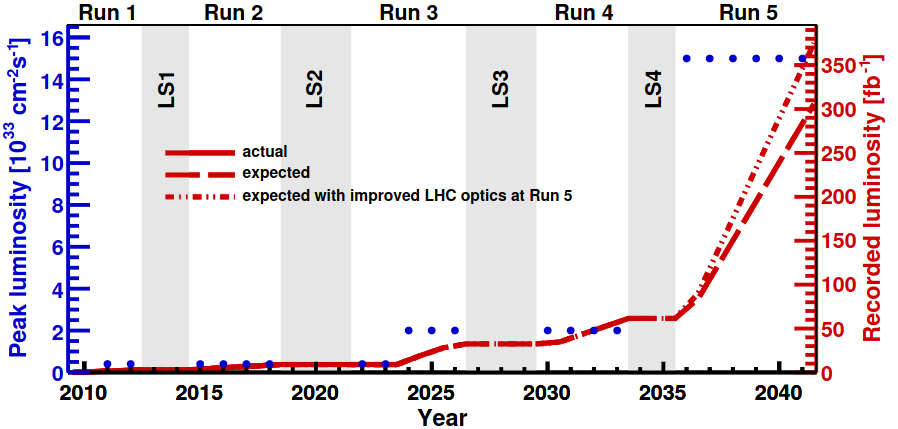
\includegraphics[width=0.7\linewidth]{figs/Luminosity.png}
    \caption[Instantaneous (peak) and integrated (recorded) luminosity profiles]{Instantaneous (peak) and integrated (recorded) luminosity for the original LHCb (Runs 1 and 2), Upgrade I (Runs 3 and 4) and the Upgrade II (Run 5) detectors.\cite{LHCbcollaboration:2903094}}
    \label{fig:luminosity}
\end{figure}
As a consequence, the number of visible pp interactions per bunch crossing will increase from about $\numrange{6}{40}$. This increased pile-up leads to a much higher particle multiplicity, larger detector occupancies and a stronger radiation load. Efficient reconstruction of primary and secondary vertices therefore becomes significantly more challenging~\cite{Schmitz2026-je}.\\
Under these conditions, the higher luminosity requires LHCb detector technologies that combine high granularity, radiation tolerance and precise timing information. Therefore, the LHCb Upgrade II foresees a major upgrade of essentially all subdetectors (sketch of proposed upgrade shown in \cref{fig:LHCb}).\\
In the tracking system, precise spatial information must be combined with timing information (four-dimensional tracking) to assign detector hits to the correct bunch crossing and to separate tracks from different pp interactions~\cite{Schmitz2026-je}.\par
\begin{figure}[ht!]
    \centering
    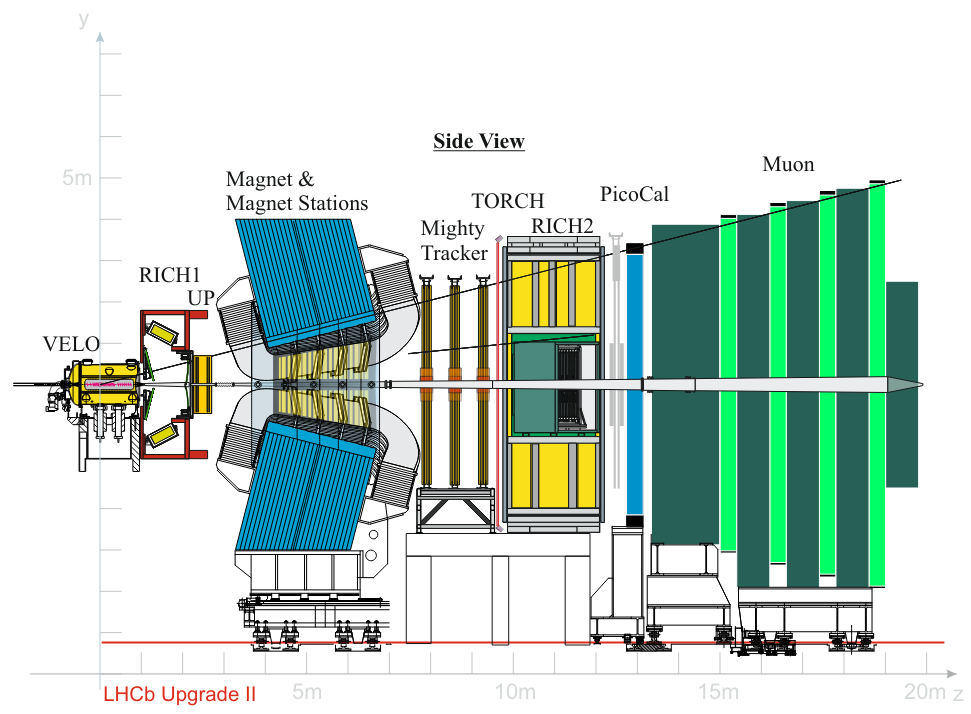
\includegraphics[width=0.7\linewidth]{figs/LHCb.png}
    \caption[Schematic side-view of LHCb]{Schematic side-view of LHCb with the proposed Upgrade II. The $y$-direction points vertically upwards and the $z$-direction points along the beamline in the direction of the subdetectors from the Vertex Locator (VELO) to the Muon detector. \cite{LHCbcollaboration:2903094}}
    \label{fig:LHCb}
\end{figure}

%
%=========================
%
\subsection{Particle Identification}
Many heavy-flavour decay channels contain charged hadrons such as pions, kaons and protons in final states with otherwise similar topologies. For example, two-body decays of the form $B\to h^+h'^-$, with $h$ denoting a charged hadron, include contributions such as $B^0\to\pi^+\pi^-$, $B_s^0\to K^+K^-$, $B^0\to K^\pm\pi^\mp$, $B_s^0\to K^\mp\pi^\pm$~\cite{2013}. Since the tracking system mainly reconstructs the trajectories and momenta of charged particles, additional particle-identification information is required to distinguish between different particle hypotheses. In the Upgrade II detector this is mainly provided by the RICH detectors, TORCH, PicoCal and the Muon system.
%
\subsubsection{RICH1 and RICH2}
The two \textbf{R}ich \textbf{I}maging \textbf{CH}erenkov detectors, RICH1 and RICH2, are used to identify charged hadrons over a broad momentum range. Using the Cherenkov effect, if a charged particle traverses a medium faster than the speed of light in that medium, it emits photons on a cone around its trajectory. The opening angle of this cone depends on the particle velocity and the refractive index of the medium. Combining this velocity information with the momentum measured by the tracking system allows the particle mass and therefore the particle type to be derived.\par
The LHCb detector uses two RICH detectors to cover different momentum regions: RICH1 is located upstream of the magnet and is optimized for lower to medium particle momenta, while RICH2 is located downstream of the magnet and covers higher momenta~\cite{2013}.
%
\subsubsection{TORCH}
TORCH, the \textbf{T}ime \textbf{O}f internally \textbf{R}eflected \textbf{CH}erenkov, is a planned time-of-flight detector for the Upgrade II detector. It is designed to improve the identification of low-momentum charged hadrons. Charged particles traversing the quartz radiator produce Cherenkov photons. These photons propagate through the quartz plate by total internal reflection and are detected at the edge of the plate by fast photon detectors. From the photon arrival time and the reconstructed track information, the particle time of flight can be determined.\par
This timing information is particularly useful for separating pions, kaons and protons at low momentum, where RICH information alone is less effective, therefore complementing it~\cite{CERN-LHCC-2021-012}.
%
\subsubsection{PicoCal}
PicoCal is the electromagnetic calorimeter foreseen for the Upgrade II detector. Its main purpose is the reconstruction and identification of electromagnetic particles such as photons, electrons and positrons. In a calorimeter, incident particles deposit their energy in an absorber material and generate a particle shower. Measuring the deposited energy and the shower shape allows electromagnetic particles to be distinguished by hadrons.\par
Under Upgrade II conditions, the calorimeter must operate at higher particle rates and occupancies, hence the importance on improved granularity and timing information for the separation of nearby showers and association of energy deposits with the correct pp interaction~\cite{CERN-LHCC-2021-012}.
%
\subsubsection{Muon System}
A staple of all detectors at LHC is the Muon system, which at the LHCb experiment is located at the end of the beamline. Since Muons are highly penetrating particles and can traverse the calorimeter and absorber material more easily than most hadrons, the muon system provides important information for identifying muons in the final state. Due to the increased particle rate under Upgrade II conditions, a higher granularity and possibly additional shielding is required to maintain efficient muon identification in the central high-rate region~\cite{CERN-LHCC-2021-012}.
%
%=========================
%
\subsection{Tracking and Momentum Reconstruction}
Tracking denotes the reconstruction of charged-particle trajectories from spatial measurements in several detector layers. In LHCb, the tracking system is pivotal for vertex reconstruction, decay-time measurements, momentum determination and the rejection of fake tracks. Since heavy-flavour particles often travel a measurable distance before decaying, a precise tracking system is needed to distinguish the primary vertex of the pp interaction from displaced secondary vertices.
%
\subsubsection{Vertex Locator (VELO)}
The \textbf{VE}rtex \textbf{LO}cator (VELO) is the tracking detector closest to the interaction point. Its main task is the precise reconstruction of charged-particle tracks close to the pp collision region. This allows the primary collision vertices and displaced secondary decay vertices to be reconstructed with high precision. The latter are especially important for identifying decays of beauty and charm hadrons.\par
For the Upgrade II, VELO must operate in an environment with higher track density and radiation load. In addition to precise spatial measurements, fast timing information is required to assign tracks to the correct interaction in the high pile-up environment~\cite{Schmitz2026-je}\cite{CERN-LHCC-2021-012}.
%
\subsubsection{Magnet and Magnet Stations}
The LHCb dipole magnet bends charged particles in the detector acceptance. Since the curvature of a charged-particle trajectory in a magnetic field depends on its momentum, the magnet is essential for momentum reconstruction. Tracking detectors before and after the magnet measure the particle trajectory, from which the momentum can be determined.\par
In the upcoming upgrade, additional Magnet Stations are foreseen inside the magnet region. Their purpose is to improve on the reconstruction of low-momentum particles that are bent strongly by the magnetic field and may not reach the downstream tracking system. The Magnet Stations therefore extend the tracking acceptance and improve the momentum determination for particles that would otherwise be poorly reconstructed or lost~\cite{CERN-LHCC-2021-012}.
%
\subsubsection{Mighty Tracker}
Since the work performed in this thesis serves the further development of the downstream tracking stations, a more in-depth discussion is given in the following~\Cref{sec:mighty_tracker}.
%
%====================================================
%
\section{Mighty Tracker}\label{sec:mighty_tracker}
The downstream tracking system is one of the central components of the LHCb detector. It is located downstream of the dipole magnet and provides the spatial measurements required to reconstruct charged-particle trajectories after their deflection in the magnetic field. Under Upgrade II conditions, the downstream tracker has to operate in a significantly harsher environment than during the present LHCb running periods. The increased instantaneous luminosity leads to much higher particle rates, larger occupancies and an increased radiation damage. In particular, the central region close to the beam pipe becomes too demanding for a purely scintillating-fibre-based tracking system used in the current detector. For this reason, the downstream tracker will be upgraded to the Mighty Tracker, a hybrid detector combining scintillating fibres in the outer region with silicon pixel detectors in the central high-occupancy region\cite{Schmitz2026-je}.
%
\subsection{Motivation for the Downstream-Tracker Upgrade}\label{sec:motivation_upgrade}
The present downstream tracking system is based on scintillating fibres (SciFi). This technology is well suited for covering large detector areas with comparatively low material budget. Charged particles crossing the fibres produce scintillation light, which is transported along the fibres and detected by silicon photomultipliers. This way the current SciFi detector provides efficient large-area tracking and is a successful choice for the present detector environment~\cite{Schmitz2026-je}\cite{DeFreitasCarneiroDaGraca:2924059}.\par
However, the Upgrade II luminosity changes the operating conditions substantially. The central part of the tracker is expected to experience particle rates of up to $\SI{17}{\mega\hertz\per\square\centi\meter}$ and hit rates of up to approximately $\SI{34}{\mega\hertz\per\square\centi\meter}$~\cite{VilellaFigueras2025-maps}. In addition, the innermost region must tolerate radiation levels of the order of $\SI{3e14}{\mega\electronvolt\per\square\centi\meter}$ (NIEL\footnote{Non-ionizing energy loss, i.e. energy deposited in the sensor material through displacement damage.}) and $\SI{40}{\mega\rad}$ (TID\footnote{TID denotes the total ionizing dose and describes the accumulated ionizing radiation dose, mainly relevant for charge build-up in insulation layers.})~\cite{VilellaFigueras2025-maps}. These values exceed the conditions for which a purely fibre-based tracker is suitable.\par
The main limitation is occupancy. If too many particles cross the same fibre region within one event, the number of possible hit combinations grows strongly. This leads to ambiguous track reconstruction and a large ghost rate. A ghost track is a reconstructed track that does not correspond to a real charged particle, but instead arises from unrelated hits that accidentally form a track-like pattern. Operating the current SciFi design under Upgrade II conditions would lead to an almost fully saturated ghost rate in the central region, making efficient charged-particle tracking impossible~\cite{Schmitz2026-je}.
%
\subsection{Hybrid Mighty Tracker Concept}
The Mighty Tracker is designed as a hybrid downstream tracking detector. It consists of two complementary detector technologies: the \textit{Mighty-SciFi} in the outer region and the \textit{Mighty-Pixel} in the central region close to the beam pipe (\cref{fig:MightyTracker}).
\begin{figure}[ht]
    \centering
    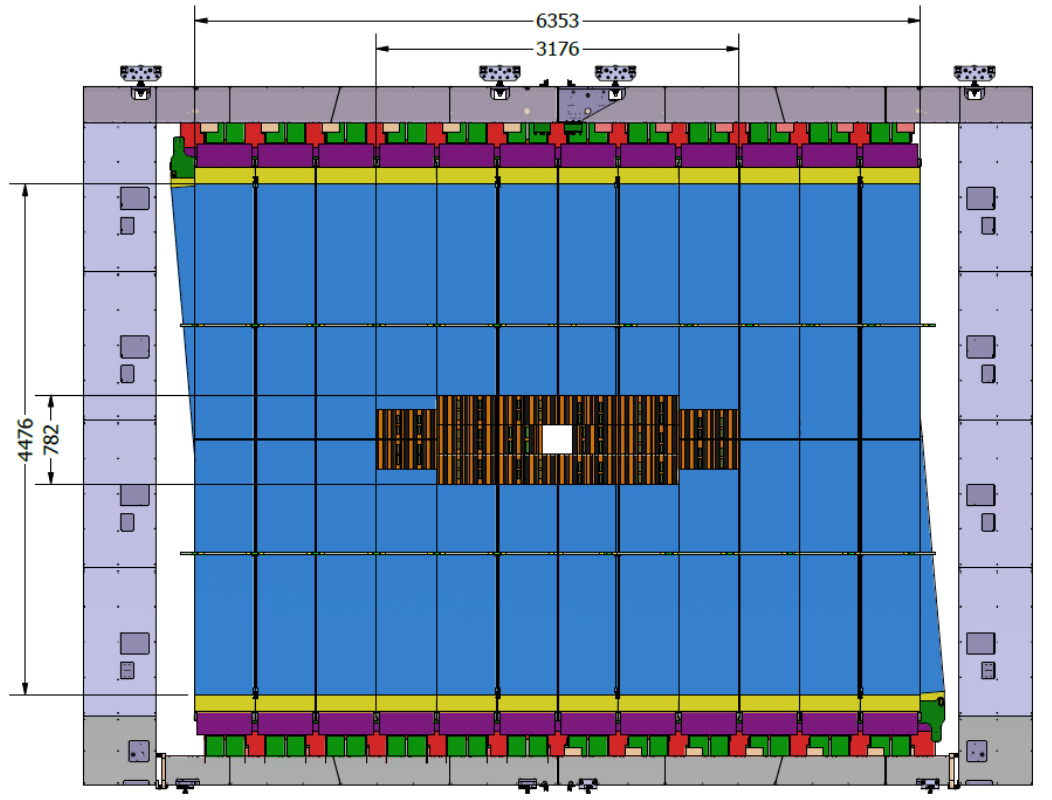
\includegraphics[width=0.7\linewidth]{figs/MightyPixel.png}
    \caption[Mighty Tracker (front view)]{Rendering of the Mighty Tracker with fibre modules (blue) in the outer regions of the detector and silicon pixel modules (brown) in the central region. The detector is held in place by C-frames (gray) with the readout electronics at the top and bottom indicated~\cite{CERN-LHCC-2021-012}}
    \label{fig:MightyTracker}
\end{figure}
The outer region covers a large area but has comparatively lower particle occupancy. In this region, SciFi remains a cost- and material-efficient solution. The central region however is exposed to the highest particle rates and radiation levels in which silicon pixel detectors provide the required granularity, radiation tolerance and timing capability. The Mighty Tracker follows the general structure of the present downstream tracker with three tracking stations and several tracking layers each. The silicon part is arranged according to the expected occupancy distribution, which is influenced by the beam geometry and the bending of particles in the LHCb magnet~\cite{CERN-LHCC-2021-012}.
%
\subsubsection{Mighty-SciFi}
The Mighty-SciFi is the scintillating-fibre part of the Might Tracker. Its role is to cover the large outer region of the downstream tracker, where occupancy remains low enough for fibre-based tracking. Three double layers with different stereo orientations ($\pm \SI{5}{\degree}$ for the inner layers) are used to reconstruct two-dimensional hit positions and suppress fake track combinations~\cite{Schmitz2026-je}. Since the outer detector area is large, using silicon pixels everywhere would be an expensive endeavour and introduce unnecessary complexity, which is why the Mighty-SciFi remains the appropriate technology for the outer acceptance~\cite{CERN-LHCC-2021-012}.\par
Nevertheless, the increased radiation load, particularly affecting the readout silicon photomultipliers (SiPMs), requires further improvements to these technologies and cooling to cryogenic temperatures~\cite{SciFi}\cite{Ronchetti:2920254}.
%
\subsubsection{Mighty-Pixel}
The Mighty-Pixel is the silicon-pixel part for the Mighty Tracker. It covers the central high-occupancy region around the beam pipe, where the hit density is too large for SciFi. The main purpose of the Mighty-Pixel is to provide high granularity tracking information with sufficient timing precision and radiation tolerance.\par
The relevant requirements, in addition those mentioned in \Cref{sec:motivation_upgrade}, include a power consumption limited to roughly $\SI{150}{\milli\watt\per\square\centi\meter}$ and a time resolution of $\leq\SI{3}{\nano\second}$\footnote{The LHC bunch crossing frequency is $\SI{40}{\mega\hertz}$, corresponding to a time separation of $\SI{25}{\nano\second}$ between consecutive bunch crossings. A time resolution of $\sim\SI{3}{\nano\second}$ allows a $\pm 4\sigma$ timing window of about $\SI{24}{\nano\second}$, which fits within one bunch-crossing interval. For a Gaussian timing response, this corresponds to an in-time efficiency of about $\SI{99.99}{\percent}$, meaning that nearly all hits are assigned to the correct bunch crossing.}~\cite{CERN-LHCC-2021-012}.\par
These requirements motivate the use of High-Voltage Monolithic Active Pixel Sensors (HV-MAPS). They combine the sensing volume and readout electronics in one monolithic silicon chip and can provide fast charge collection by drift in a depleted region. The production sensor family developed for the Might-Pixel is called MightyPix with the current MightyPix2 as an intermediate development step toward the final production sensor.
%
\subsection{Mighty-Pixel Layout}

\begin{figure}[ht]
    \centering
    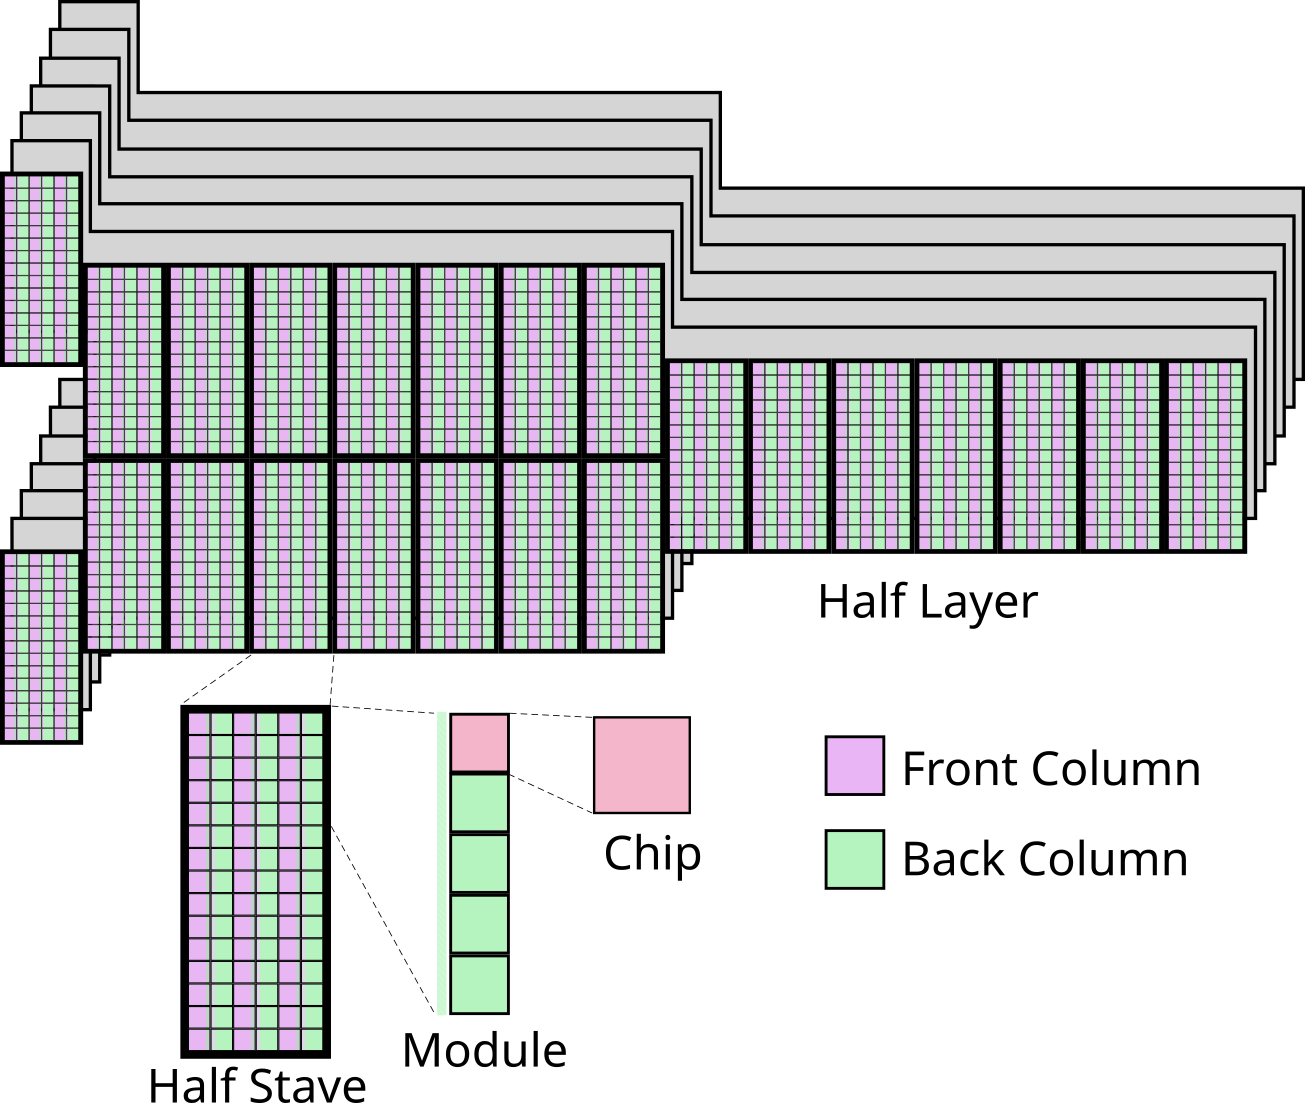
\includegraphics[width=0.7\linewidth]{figs/MP_sketch2.png}
    \caption{Caption}
    \label{fig:placeholder}
\end{figure}
\begin{figure}[ht]
    \centering
    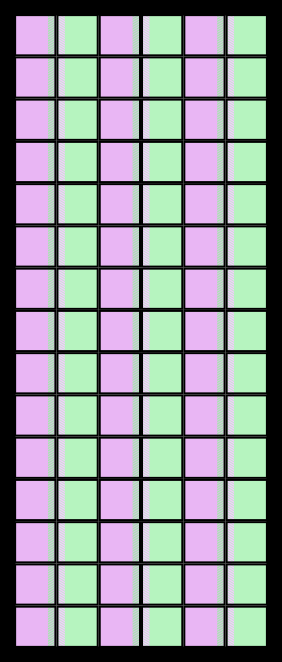
\includegraphics[width=0.1\linewidth]{figs/half_stave.png}
    \caption{Caption}
    \label{fig:placeholder}
\end{figure}
%
\subsection{Module and Stave Architecture}
\begin{figure}[ht]
    \centering
    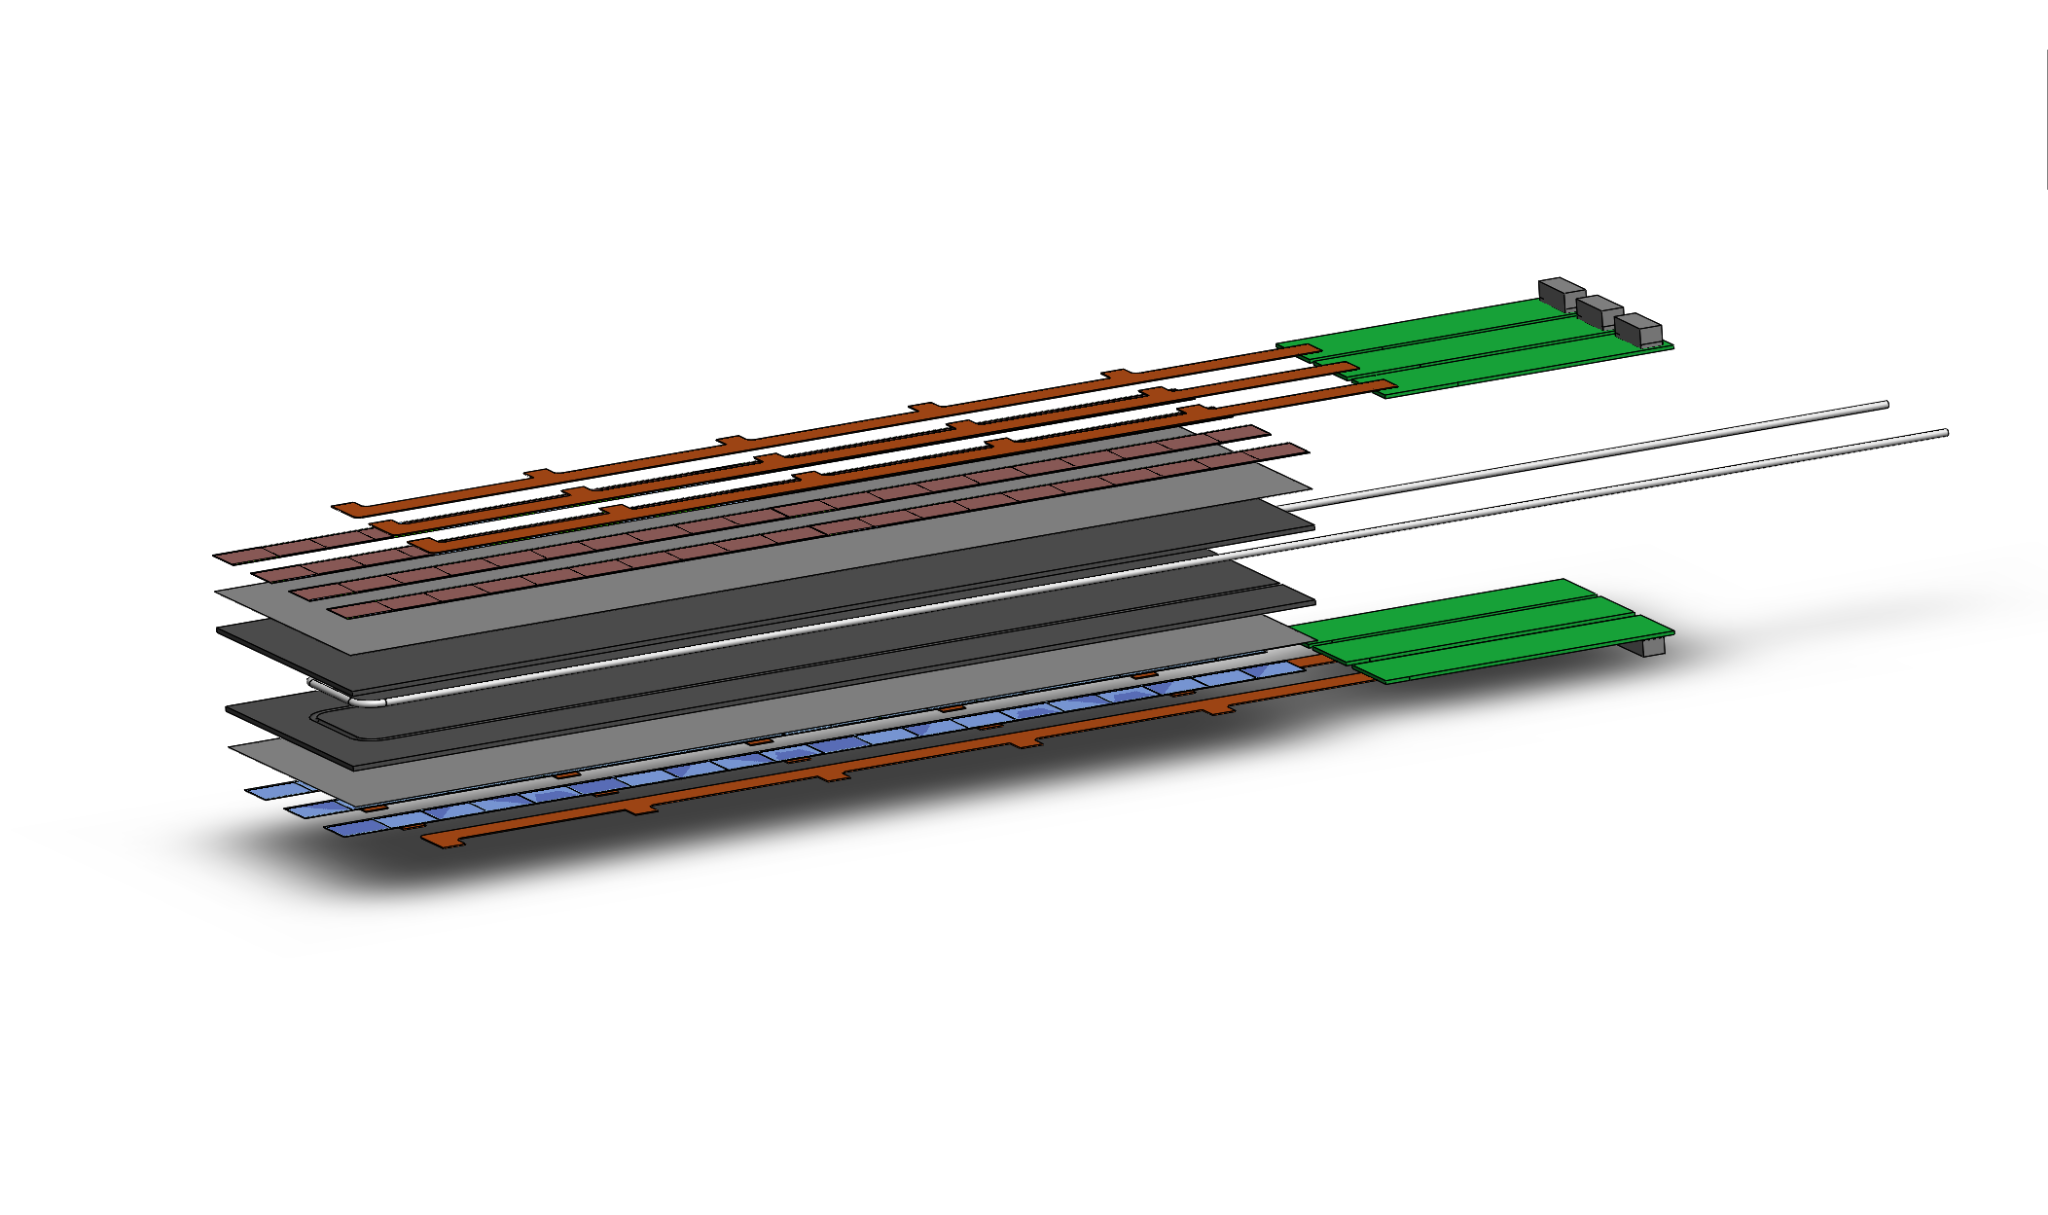
\includegraphics[width=0.7\linewidth]{figs/Stave.png}
    \caption{Caption}
    \label{fig:placeholder}
\end{figure}
\begin{figure}[ht]
    \centering
    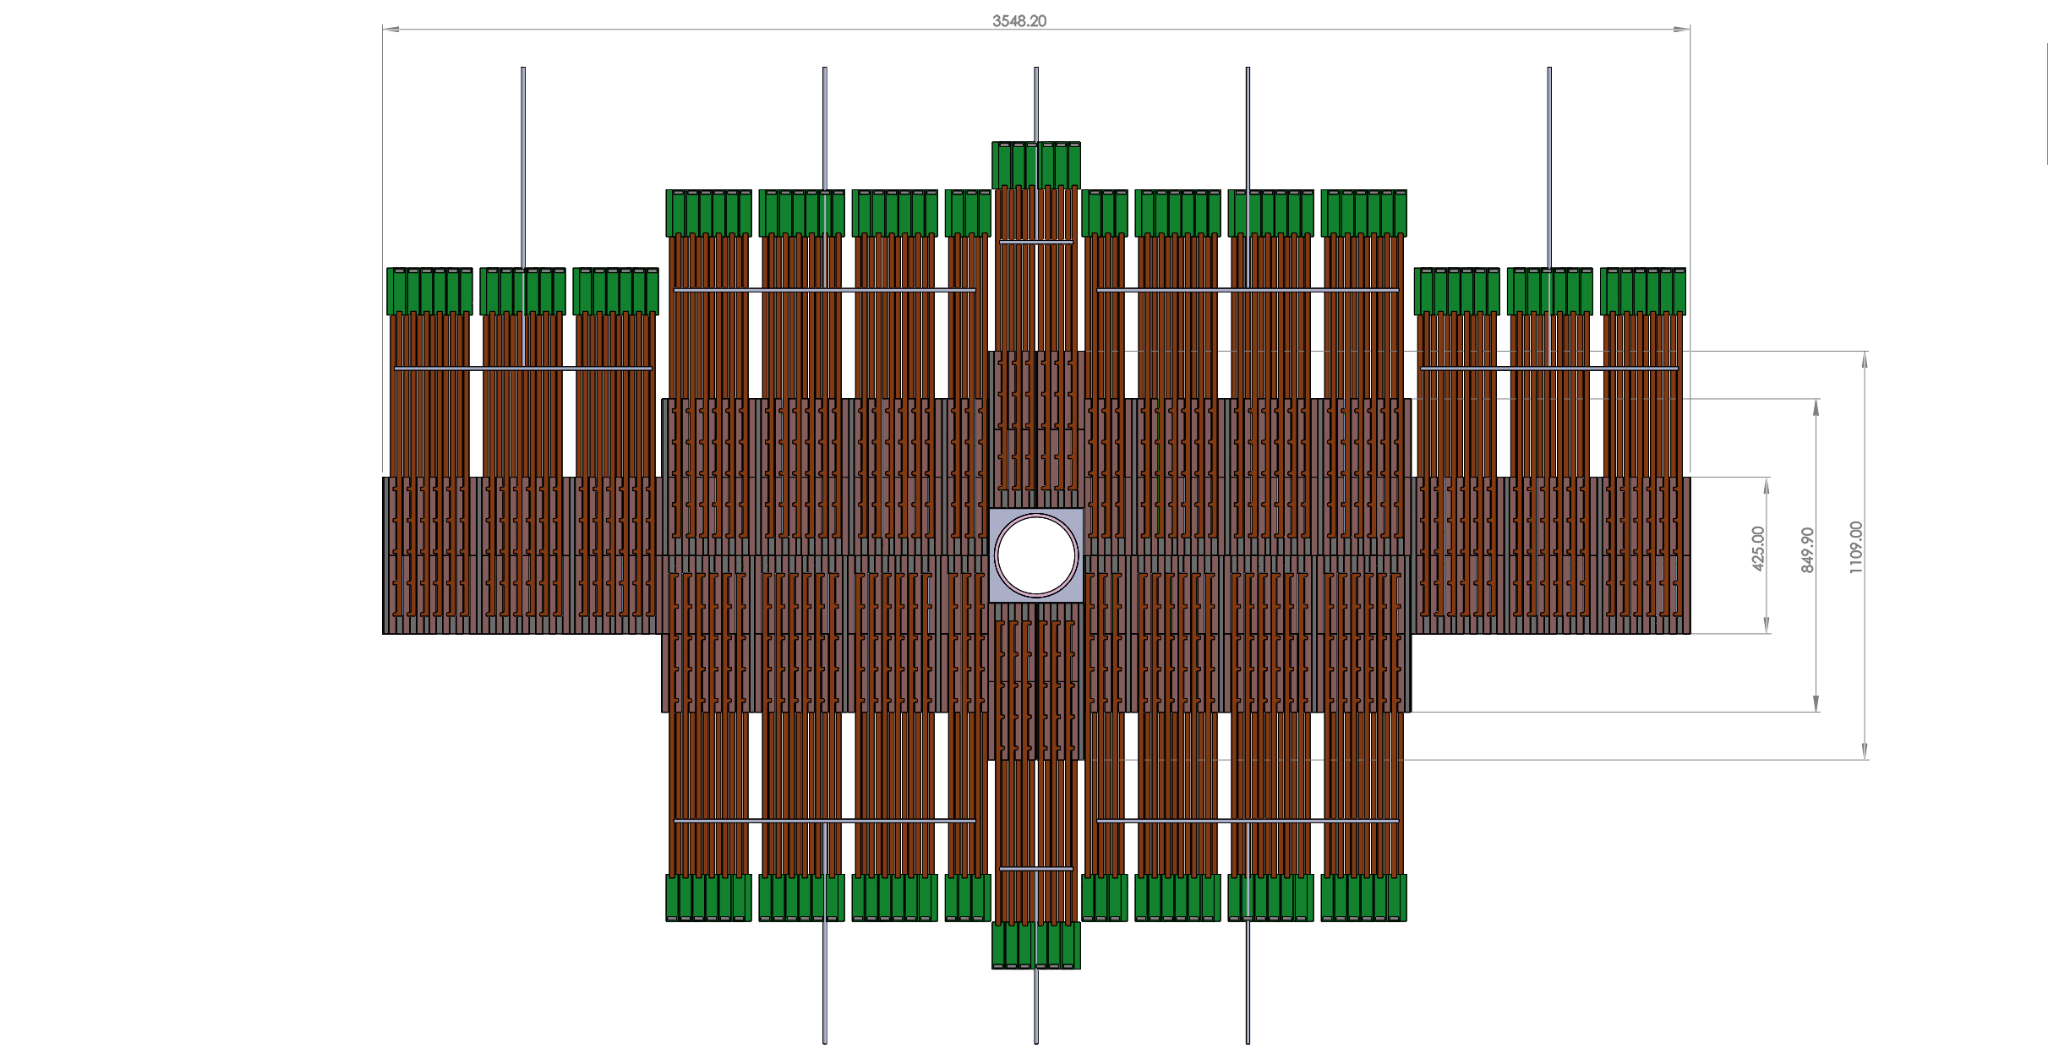
\includegraphics[width=0.7\linewidth]{figs/StaveBuildOverview.png}
    \caption{Caption}
    \label{fig:placeholder}
\end{figure}
%
\subsection{MightyPix2 and HV-MAPS}

%
\subsubsection{High-Voltage CMOS Principle}
\begin{figure}[ht]
    \centering
    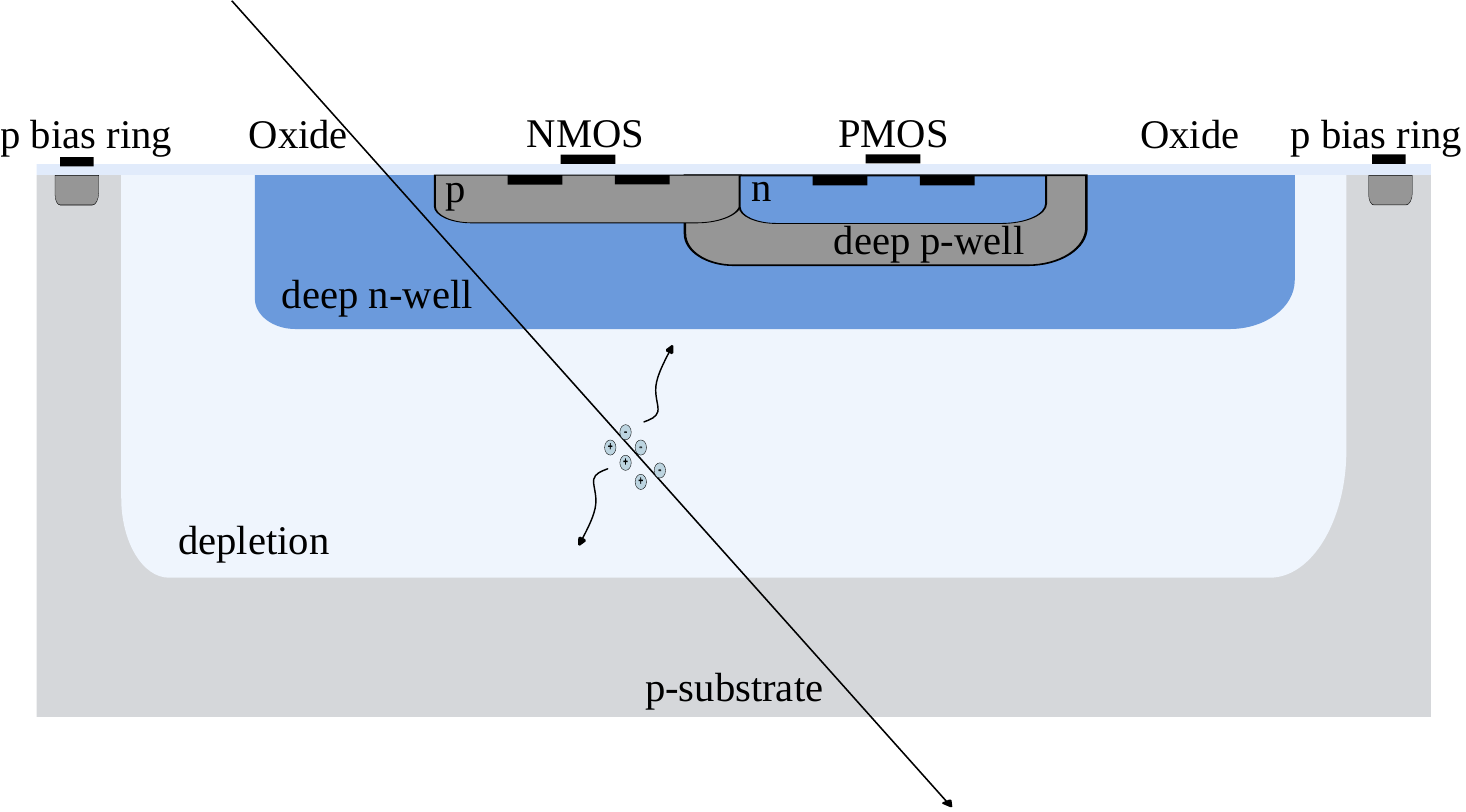
\includegraphics[width=0.7\linewidth]{figs/HVCMOS.png}
    \caption{Caption}
    \label{fig:placeholder}
\end{figure}
\begin{figure}[ht]
    \centering
    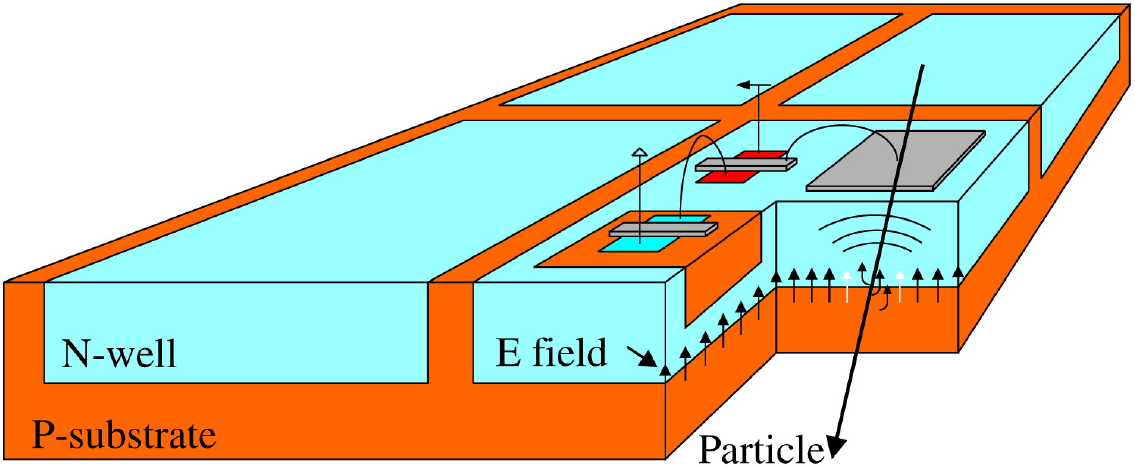
\includegraphics[width=0.7\linewidth]{figs/HVMAPS.png}
    \caption{Caption}
    \label{fig:placeholder}
\end{figure}
%
\subsubsection{Charge Collection and Timing}
%
\subsubsection{MightyPix2 Design}
%
\subsection{Positioning Problems}
%
\subsubsection{Sensor-to-Sensor Spacing}
%
\subsubsection{Sensor-to-Support Insulation}
\begin{figure}[ht]
    \centering
    \subcaptionbox{}{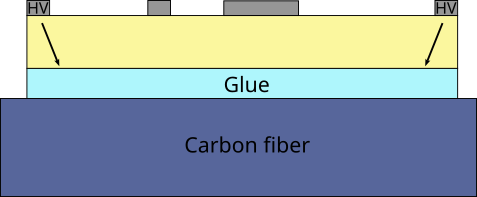
\includegraphics[width=0.49\linewidth]{figs/chip_carbon_nopas.png}}
    \subcaptionbox{}{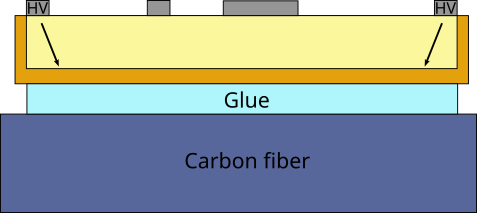
\includegraphics[width=0.49\linewidth]{figs/chip_carbon_pas.png}}
    \caption{Caption}
    \label{fig:placeholder}
\end{figure}
